\documentclass{cpereport}
\usepackage{tikz}
\usepackage{amsmath}
\usepackage{amssymb}
\usepackage{mathrsfs}
\usepackage{hyperref}
\usepackage{pgfplots}
\usepackage{tcolorbox}
\usepackage{xcolor}
\usepackage{enumitem}

\definecolor{mat-blue-200}{HTML}{e3f2fd}
\definecolor{mat-blue-900}{HTML}{2286c3}
\definecolor{mat-teal-50}{HTML}{e0f2f1}
\definecolor{mat-teal-900}{HTML}{004d40}
\definecolor{mat-bg-50}{HTML}{eceff1}
\definecolor{mat-bg-900}{HTML}{37474f}

\newtcolorbox{info-box}{
    colback=mat-blue-200,
    colupper=mat-blue-900,
    colframe=mat-blue-900,
    boxrule=1pt,
    width=\textwidth
}
\newtcolorbox{success-box}{
    colback=mat-teal-50,
    colupper=mat-teal-900,
    colframe=mat-teal-900,
    boxrule=1pt,
    width=\textwidth
}
\newtcolorbox{dark-box}{
    colback=mat-bg-50,
    colupper=mat-bg-900,
    colframe=mat-bg-900,
    boxrule=1pt,
    width=\textwidth
}
\newtcolorbox{plain-box}{
    colback=white,
    colupper=black,
    colframe=black,
    boxrule=1pt,
    wide=\textwidth
}

\begin{document}

\tableofcontents

\chapter{บทนำ}

\section{ความเป็นมาและความสําคัญของปัญหา}

แบบจำลองจักรกลเรียนรู้ (Machine Learning models) นั้นถูกใช้อย่างกว้างขวางในปัจจุบัน อย่างไรก็ตาม แบบจำลองใดๆ นั้นอาจมีความผิดพลาดต่อการทำการโจมตีประสงค์ร้าย (Adversarial attacks) เพื่อจงใจให้ผลลัพธ์ที่แบบจำลองนั้นคาดเดามีความผิดพลาดจากผลลัพธ์ที่ควรจะเป็น

ในการเรียนรู้เชิงตัวแปรเสริม (parameter-based learning) นั้น ตัวแปรเสริม (parameters) ค่าน้ำหนัก (weights) บนแบบจำลองการเรียนรู้เชิงลึก (deep Learning models) เป็นตัวกำหนดความฉลาดของแบบจำลอง อาจมีตัวแปรเสริมบางชุดที่ทำให้แบบจำลองมีช่องโหว่ต่อการโจมตีประสงค์ร้าย การโจมตีนั้นอาจเกิดจากการเพิ่มสัญญาณรบกวนซึ่งผ่านการคำนวน (calculated artefacts) เข้าสู่ข้อมูลรับเข้า (inputs) ซึ่งทำให้ความผิดพลาดของแบบจำลองในการพยากรณ์คำตอบนั้นเปลี่ยนไปอย่างชัดเจน 

โครงงานวิศวกรรมคอมพิวเตอร์นี้มุ่งหวังจะนำตัวแปรเสริมบนแบบจำลองมาสร้างภาพแสดง (visualise) ถึงจุดโหว่ในการพยากรณ์ใดๆ ของแบบจำลอง เพื่อลดความเสียหายอันอาจเกิดขึ้นได้จากการโจมตีแบบจำลองขณะถูกใช้งานจริง

\section{วัตถุประสงค์ของการศึกษา}
\noindent
โครงงานนี้มีวัตถุประสงค์และเป้าหมายดังนี้

\begin{enumerate}
    \item สร้างแบบจำลองเชิงลึก (Deep Learning models) ซึ่งสามารถถูกโจมตีประสงค์ร้าย (Adversarial attacks) ได้
    \item นำแบบจำลองในข้อ (1) มาสร้างเป็นรูปภาพแสดง (visualisation) เพื่อหาจุดโหว่ต่อการโจมตี รวมถึงคาดเดาแนวโน้มการโจมตีที่เป็นไปได้
    \item ใช้ความรู้ในข้อ (2) สร้างแบบจำลองที่ทนทาน (prone) ต่อการโจมตีมากขึ้น
\end{enumerate}

\section{ขอบเขตของการทําโครงงาน}
\noindent
โครงงานนี้มีขอบเขตการดำเนินงานดังนี้

\begin{enumerate}
    \item สร้างแบบจำลองเชิงลึก (Deep Learning models) ซึ่งสามารถถูกโจมตีประสงค์ร้าย (Adversarial attacks) ได้
    \item นำแบบจำลองในข้อ (1) มาสร้างเป็นรูปภาพแสดง (visualisation) เพื่อหาจุดโหว่ต่อการโจมตี รวมถึงคาดเดาแนวโน้มการโจมตีที่เป็นไปได้
    \item ใช้ความรู้ในข้อ (2) สร้างแบบจำลองที่ทนทาน (prone) ต่อการโจมตีมากขึ้น
\end{enumerate}

\section{ระยะเวลาและแผนดําเนินงาน}
การดำเนินงานของโครงการจะใช้วิธีจัดการงาน (workflow) แบบเอไจล์ (agile) เพื่อมุ่งเน้นประสิทธิภาพในการทำงานและสร้างระบบการทำงานที่เหมาะสมต่อการดำเนินการในระยะเวลาและปัจจัยการดำเนินงานที่ไม่อาจคาดเดาได้
การทำงานจะใช้วิธีการแบ่งรอบการวนทวน (iteration) โดยมุ่งเน้นให้แต่ละรอบการวนทวนมีความก้าวหน้าของงานในปริมาณที่เหมาะสมกับเวลาและข้อจำกัดต่างๆ
หนึ่งรอบการวนทวนนั้นกินระยะเวลาสองสัปดาห์ดังแสดงในตารางที่ \ref{iteration-timetable} และจะประกอบด้วยขั้นตอนต่อไปนี้
\begin{enumerate}
    \item ประชุมสรุป (iteration meeting) หนึ่งถึงสองครั้งต่อสัปดาห์
    \item เขียนรอบปูมย้อนหลัง (backlog) และหยิบมาทำตามจำนวนที่เหมาะสม
    \item กิจกรรมมองย้อนรอบการวนทวนด้วยตนเอง (self-retrospective) เพื่อพิจารณาความเหมาะสมในการทำงาน และปรับปรุงการทำงานในรอบการวนทวนต่อไป
\end{enumerate}
อย่างไรก็ดี เพื่อเป็นการตั้งเป้าหมายงานในระยะยาว โครงงานนี้จะมีวิสัยทัศน์ผลิตภัณฑ์ (product vision) โดยคร่าวตามขอบเขตการดำเนินงาน และในทุกประมาณ 4-6 รอบการวนทวน จะมีการวางแผนปล่อยผลิตภัณฑ์ (release planning) หนึ่งครั้งเพื่อสรุปงานออกมาเป็นความคืบหน้าที่จับต้องได้อันเกิดจากการทำงานในกลุ่มรอบการวนทวนนั้น

\begin{table}[]
    \centering
    \begin{tabular}{r|cccc|ccc}
    \hline \hline
     & \multicolumn{4}{c|}{2562} & \multicolumn{3}{c}{2563} \\
     & ก.ย. & ต.ค. & พ.ย. & ธ.ค. & ม.ค. & ก.พ. & มี.ค. \\ \hline
    รอบการวนทวนที่ 1 & / &  &  &  &  &  &  \\
    รอบการวนทวนที่ 2 & / &  &  &  &  &  &  \\
    รอบการวนทวนที่ 3 &  & / &  &  &  &  &  \\
    รอบการวนทวนที่ 4 &  & / &  &  &  &  &  \\
    รอบการวนทวนที่ 5 &  &  & / &  &  &  &  \\
    รอบการวนทวนที่ 6 &  &  & / &  &  &  &  \\
    แผนการปล่อยงานที่ 1 &  &  & / &  &  &  &  \\
    รอบการวนทวนที่ 7 &  &  &  & / &  &  &  \\
    รอบการวนทวนที่ 8 &  &  &  & / &  &  &  \\
    รอบการวนทวนที่ 9 &  &  &  &  & / &  &  \\
    รอบการวนทวนที่ 10 &  &  &  &  & / &  &  \\
    แผนการปล่อยงานที่ 2 &  &  &  &  & / &  &  \\
    รอบการวนทวนที่ 11 &  &  &  &  &  & / &  \\
    รอบการวนทวนที่ 12 &  &  &  &  &  & / &  \\
    รอบการวนทวนที่ 13 &  &  &  &  &  &  & / \\
    รอบการวนทวนที่ 14 &  &  &  &  &  &  & / \\
    แผนการปล่อยงานที่ 3 &  &  &  &  &  &  & / \\
    \hline \hline
    \end{tabular}
    \caption{ตารางแสดงรอบการวนทวนและช่วงเวลา}
    \label{iteration-timetable}
\end{table}

\section{ประโยชน์ที่คาดว่าจะได้รับ}
\begin{enumerate}
    \item เข้าใจถึงพื้นฐาน หลักการทำงาน และระบบจักรกลเรียนรู้แบบต่างๆ
    \item เข้าใจถึงจุดอ่อนของระบบจักรกลเรียนรู้ในแต่ละกรณี
    \item สามารถโจมตีระบบจักรกลเรียนรู้ เพื่อสร้างระบบจักรกลเรียนรู้ที่ทนทานต่อการโจมตีได้
\end{enumerate}

\section{คํานิยามศัพท์เฉพาะ}
\begin{itemize}
    \item \textbf{จักรกลเรียนรู้} (machine learning) คือระบบ หรือโค้ด หรือโปรแกรมคอมพิวเตอร์ที่เรียนรู้โครงสร้างของชุดคำถามและคำตอบโดยมิจำเป็นต้องทำการโปรแกรมลำดับการทำงานอย่างชัดแจ้ง (explicitly) 
    \item \textbf{การเรียนรู้เชิงโจมตี} (adversarial learning) หมายถึงการศึกษาถึงการโจมตีแบบจำลอง (model) ของจักรกลเรียนรู้ (machine learning)
\end{itemize}

\chapter{ทฤษฎีและงานวิจัยที่เกี่ยวข้อง}
\section{จักรกลเรียนรู้}
ระบบจักรกลเรียนรู้ (machine learning) อาจนิยามได้ว่าเป็นระบบที่ไม่ต้องมีการป้อนข้อมูล หรือวิธีทำงาน เข้าไปยังโค้ดโปรแกรมอย่างชัดแจ้ง (explicitly) โดยระบบดังกล่าวจะถูกฝึกสอนด้วยชุดของข้อมูลหรือประสบการณ์ (experience) และปรับตัวเองให้ส่งออกคำตอบซึ่งอิงจากประสบการณ์ที่ตนเองเคยได้เรียนรู้มา

หากจะกล่าวให้ละเอียด เราสามารถนิยามโปรแกรมซึ่งสามารถทำการ\textit{เรียน}ได้ดังนี้ \cite{Mitchell97}

\begin{definition}
โปรแกรมใดๆ เรียน (learn) จากประสบการณ์ (experience) $E$ บนงาน (task) $T$ และการวัดประสิทธิผล (performance measurement) $P$ หากประสิทธิผลบน $T$ ซึ่งถูกวัดโดย $P$ เพิ่มขึ้นตามประสบการณ์ $E$
\end{definition}

\section{การเรียนรู้เชิงลึก}
การเรียนรู้เชิงลึก (Deep Learning) คือความพยายามในการจำลองเซลล์ประสามของมนุษย์ให้อยู่ในรูปแบบจำลองคณิตศาสตร์
ด้วยความเชื่อทางหลักประสาทวิทยา (neurosciences) ว่าความฉลาดของสมองมนุษย์เกิดขึ้นได้จากโครงข่ายประสาทจำนวนมาก
ที่เชื่อมเข้าถึงกัน \cite{Goodfellow-et-al-2016}

\subsection{เปอร์เซปตรอน (Perceptron)}
\begin{figure}
    \centering
    \begin{tikzpicture}
        \def\layersep{2cm}
        \tikzstyle{neuron}=[circle,draw=black!100,minimum size=24pt, outer sep=3pt]
        \tikzstyle{annot}=[text width=5em, text centered]
        
        \node[neuron, pin=left:อคติ $b$] (bias) at (0, 0cm) {$w_0$};
        \foreach \name / \y in {1,...,3}
            \node[neuron, pin=left: ข้อมูลรับเข้า $x_\y$] (I-\name) at (0,-\y) {$w_\y$};
    
        \node[annot] (I-h) at (0, -4) {$\vdots$};
        \node[neuron, pin=left:ข้อมูลรับเข้า $x_n$] (I-4) at (0,-5) {$w_n$};

        \node[neuron] (sum) at (1*\layersep,-2 cm) {$\Sigma$};
        \node[neuron] (activation) at (3.75*\layersep,-2 cm) {$\sigma$};

        \foreach \source in {1,...,4}
            \draw [->] (I-\source) -- (sum);
        \draw [->] (bias) -- (sum);
        \draw [->] (sum) -- (activation) node [midway, above] (SumDesc) {$s = \left(\sum_{i=1}^{N} w_ix_i\right) + w_0$};
        \draw [->] (activation) -- (5.5*\layersep, -2cm) node [midway, above] (ActDesc) {ส่งออก $y = \sigma(s)$};
    \end{tikzpicture}
    \caption{เปอร์เซปตรอน}
    \label{tikz-perceptron}
\end{figure}
เปอร์เซปตรอน (Perceptron) \cite{rosenblatt_1958} เป็นแบบจำลองทางคณิตศาสตร์ของเซลล์สมองหนึ่งเซลล์ โดยมีคุณสมบัติดังนี้

\begin{itemize}
    \item รับเข้าข้อมูลมาในเซลล์จากหลายแหล่ง และให้น้ำหนักกับข้อมูลนั้นต่างกันไป
    \item ส่งออกข้อมูลเพียงค่าเดียว
\end{itemize}

ดังนั้น แบบจำลองทางคณิตศาสตร์สามารถเขียนออกมาจากหลักการสองข้อดังกล่าวได้ด้วยสมการ

\begin{equation}
y = \sigma\left(W^TX+b\right)
\end{equation}

เมื่อ $W$ และ $X$ เป็นเมทริกซ์ขนาด $1 \times n$ (โดย $n$ เป็นจำนวนข้อมูลรับเข้า), $b$ เป็นค่าสัมประสิทธิ์คงที่ (อคติ: bias)
และ $\sigma$ เป็นฟังก์ชันกระตุ้น (activation function) ซึ่งอาจเขียนรูปร่างของเปอร์เซปตรอนให้มีลักษณะรูปคล้ายเซลล์สมองได้ในลักษณะรูปที่ \ref{tikz-perceptron}

ยกตัวอย่างการใช้เปอร์เซปตรอนในการแก้ปัญหาอย่างง่ายได้ในที่นี้

\subsubsection{การคาดเดาราคาอสังหาริมทรัพย์}
หากสำรวจราคาอสังหาริมทรัพย์แล้วพบว่า
\begin{itemize}
    \item ราคาอสังหาริมทรัพย์จะเพิ่มขึ้นตามที่ดิน โดยเพิ่มขึ้นทุก 10,000 บาทต่อตารางวา
    \item ราคาอสังหาริมทรัพย์จะเพิ่มขึ้นตามจำนวนห้องนอน โดยเพิ่มขึ้นทุก 200,000 บาทต่อห้องนอน
    \item ราคาอสังหาริมทรัพย์จะลดลงตามจำนวนอายุปี โดยลดลงทุก 7,000 บาทต่ออายุของอสังหาริมทัพย์
    \item ราคากำหนดตรึง (fixed cost) ของอสังหาริมทรัพย์ อยู่ที่ 100,000 บาท
\end{itemize}
\noindent
จะสามารถเขียนเปอร์เซปตรอนเพื่อคาดเดาราคาอสังหาริมทรัพย์ได้โดย
$$ y = \sigma\left(W^TX\right) $$
เมื่อ $W$ ซึ่งเป็นค่าสัมประสิทธิ์แสดงถึงความสัมพันธ์ข้อมูลรับเข้า ซึ่งเขียนได้จากความสัมพันธ์ดังแสดงด้านล่าง
$$
    W^T = \begin{bmatrix}
        100000 & 10000 & 200000 & -7000
    \end{bmatrix}
$$
หากต้องการคาดเดาราคาบ้านที่มี 3 ห้องนอน เนื้อที่ 100 ตารางวา และมีอายุ 7 ปี จะสามารถเขียนเมทริกซ์ $X$ ได้เป็น
$$
    X = \begin{bmatrix}
        1 \\
        3 \\
        100 \\
        7
    \end{bmatrix}
$$
โปรดสังเกตว่า $x_0 = 1$ เนื่องจากผลคูณของเทอม $w_0$ และ $x_0$ เป็นค่าที่เรียกว่าค่าอคติ (bias) ของแบบจำลอง

เนื่องจากเปอร์เซปตรอนตัวนี้ถูกใช้ในการทำนายราคา ซึ่งกล่าวว่ามีความสัมพันธ์กันกับตัวแปรที่กำหนดข้างต้นในเชิงเส้น ดังนั้นจะกล่าวได้ว่าฟังก์ชันกระตุ้น (activation function) ที่เลือกใช้ จะเลือกใช้ฟังก์ชันเส้นตรง (linear function) $\sigma(x) = x$

ดังนั้น ผลการทำนายราคาบ้านคำนวนได้จาก
$$
    \begin{aligned}
        y &= \sigma\left(W^TX+b\right)\\
        &= \sigma\left(\begin{bmatrix}
            100000 & 10000 & 200000 & -7000
        \end{bmatrix} \times \begin{bmatrix}
            1 \\
            3 \\
            100 \\
            7
        \end{bmatrix}\right)\\
        &= \sigma(100000 + 30000 + 20000000 + (-49000)) = f(20981000)\\
        &= 20981000
    \end{aligned}
$$

\subsubsection{การสร้างประตูสัญญาณตรรกะด้วยเปอร์เซปตรอน}
เราสามารถสร้างประตูสัญญาณตรรกะ (logic gates) บางชนิดได้ด้วยเปอร์เซปตรอน เช่นการสร้าง AND และ OR gate

ยกตัวอย่างโครงสร้างของประตูสัญญาณและซึ่งสามารถสร้างได้ด้วยการกำหนดให้
\begin{itemize}
    \item $X$ เป็นเมทริกซ์ขนาด $1 \times 2$ กล่าวคือเมื่อรับค่า $x_1, x_2$ เป็นค่า 0 หรือ 1 แทนสัญญาณจริงหรือเท็จแล้ว
        $$X = \begin{bmatrix}
            1 \\
            a_1 \\
            a_2
        \end{bmatrix}$$
    \item กำหนดค่าของเมทริกซ์ $W$ เป็น
        $$W^T = \begin{bmatrix}
            -2 & 1 & 1
        \end{bmatrix}$$
    \item กำหนดฟังก์ชัน $\sigma(x)$ เป็น step function กล่าวคือ
    $$
        \sigma(x) = \begin{cases}
            1; & x \geq 0\\
            0; & \textrm{ในกรณีอื่น}
        \end{cases}
    $$
\end{itemize}
และการสร้างประตูสัญญาณหรือสามารถทำได้ในลักษณะเดียวกันโดยเปลี่ยนชุดน้ำหนัก เป็น
        $$W^T = \begin{bmatrix}
            -1 & 1 & 1
        \end{bmatrix}$$

\subsection{เปอร์เซปตรอนแบบหลายชั้น (Multi Layer Perceptron)}

เราอาจสังเกตว่าเปอร์เซพตรอนหนึ่งตัวนั้นทำหน้าที่ได้เพียนแยก (classify) หรือถดถอย (regress) ปัญหาที่เป็นปัญหาเชิงเส้น (linear problems) ได้เท่านั้น อย่างไนก็ตามหากเรากำหนดให้ฟังก์ชัน $f$ เป็นฟังก์ชันที่ไม่ใช่ฟังก์ชันเส้นตรงแล้ว เราอาจสร้าง\textbf{เปอร์เซปตรอนแบบหลายชั้น} (Multi Layer Perceptron) ขึ้นมาได้โดยมีลักษณะดังรูปที่ \ref{mlp}

\begin{figure}
    \centering
    \def\layersep{2.5cm}
    \begin{tikzpicture}[->,draw=black!70, node distance=\layersep]
        \tikzstyle{every pin edge}=[<-,shorten <=1pt]
        \tikzstyle{neuron}=[circle,draw=black!100,minimum size=17pt, outer sep=3pt]
        \tikzstyle{annot}=[text width=5em, text centered]
    
        \foreach \name / \y in {1,...,4}
            \node[neuron, pin=left:ข้อมูลรับเข้า \y] (I-\name) at (0,-\y) {};
    
        % Draw the hidden layer nodes
        \foreach \name / \y in {1,...,5}
            \path[yshift=0.5cm]
                node[neuron] (HA-\name) at (\layersep,-\y cm) {};
    
        \foreach \name / \y in {1,...,5}
            \path[yshift=0.5cm]
                node[neuron] (HB-\name) at (2*\layersep,-\y cm) {};

        \foreach \name / \y in {1,...,3}
            \path[yshift=-0.5cm]
                node[neuron] (O-\name) at (3*\layersep,-\y cm) {};
    
        \foreach \source in {1,...,4}
            \foreach \dest in {1,...,5}
                \path (I-\source) edge (HA-\dest);
    
        \foreach \source in {1,...,5}
            \foreach \dest in {1,...,5}
                \path (HA-\source) edge (HB-\dest);

        \foreach \source in {1,...,5}
            \foreach \dest in {1,...,3}
                \path (HB-\source) edge (O-\dest);

        \node[annot,above of=I-1, node distance=1cm] (hla) {ชั้นรับเข้า (ชั้นที่ 0)};
        \node[annot,above of=HA-1, node distance=1cm] (hla) {ชั้นซ่อน 1};
        \node[annot,above of=HB-1, node distance=1cm] (hla) {ชั้นซ่อน 2};
        \node[annot,above of=O-1, node distance=1cm] (hlb) {ชั้นส่งออก (ชั้นที่ 3)};
    \end{tikzpicture}
    \caption{เปอร์เซปตรอนแบบหลายชั้น}
    \label{mlp}
\end{figure}

เราอาจเขียนแทนน้ำหนักของโครงข่ายจากเปอร์เซปตรอนชั้นที่ $i$ ไปยังชั้นที่ $j$ ($j=i+1$) ได้เป็น
\begin{equation*}
    \boldsymbol{W}_{ij} = 
    \begin{bmatrix}
        w_{10} & w_{20} & \dots & w_{n_{i}0}\\
        w_{11} & w_{21} & \dots & w_{n_{i}1}\\
        w_{12} & w_{22} & \dots & w_{n_{i}2}\\
        \vdots & \vdots & \ddots & \vdots\\
        w_{1n_j} & w_{2n_j} & \dots & w_{n_jn_i}
    \end{bmatrix}
\end{equation*}
เมื่อจำนวนเปอร์เซปตรอนในชั้นที่ $k$ เขียนแทนด้วย $n_k$

ยกตัวอย่างเช่น เราจะสามารถสร้างประตูสัญญาณเฉพาะหรือ (XOR gate) ได้จากเปอร์เซปตรอนแบบหลายชั้นดังแสดงในรูปที่ \ref{xor-mlp} โดยเลขในแต่ละเปอร์เซปตรอนแทนค่าอคติ ($b$) และเลขบนเส้นเชื่อมแทนค่าน้ำหนัก ($w$) และกำหนดให้ฟังก์ชันกระตุ้น $\sigma$ เป็นฟังก์ชันขั้นบันได (step function) กล่าวคือ
\begin{equation*}
    \sigma(x) =
    \begin{cases}
        1; & x \geq 0\\
        0; & \textrm{ในกรณีอื่น}
    \end{cases}
\end{equation*}
เปอร์เซปตรอนดังกล่าว เมื่อรับค่า $A$ และ $B$ เป็น 0 หรือ 1 จะส่งออกค่า $A \oplus B$

\begin{figure}
    \def\layersep{2.5cm}
    \centering
    \begin{tikzpicture}[<-, draw=black!70, node distance=\layersep]
        \tikzstyle{edge}=[->,fill=white]
        \tikzstyle{neuron}=[circle,draw=black!100,minimum size=25pt, outer sep=3pt]
        \tikzstyle{annot}=[text width=5em, text centered]
    
        \node[neuron, pin=left:$A$] (I-1) at (0,0 cm) {$A$};
        \node[neuron, pin=left:$B$] (I-2) at (0,-2 cm) {$B$};
    
        \node[neuron] (HA-1) at (\layersep,-0 cm) {$-2$};
        \node[neuron] (HA-2) at (\layersep,-2 cm) {$-2$};

        \node[neuron] (O) at (2*\layersep,-1 cm) {$-1$};

        \path[edge]
            (I-1) edge node {$-1$} (HA-1)
            (I-1) edge node[very near end] {$1$} (HA-2)
            (I-2) edge node[very near end] {$1$} (HA-1)
            (I-2) edge node {$-1$} (HA-2)
            (HA-1) edge node {$1$} (O)
            (HA-2) edge node {$1$} (O)
        ;
    \end{tikzpicture}
    \caption{เปอร์เซปตรอนแบบหลายชั้นซึ่งทำหน้าที่เป็นประตูสัญญาณเฉพาะหรือ}
    \label{xor-mlp}
\end{figure}

\section{ฟังก์ชันกระตุ้นและความฉลาดของโครงข่ายประสาทเทียม}
\subsection{ทฤษฎีบทตัวประมาณฟังก์ชันครอบจักรวาล}
เหตุผลที่โครงข่ายประสาทเทียมสามารถทำงานได้ดี เนื่องจากมีการพิสูจน์ว่าโครงข่ายประสาทเทียมนั้นสามารถทำหน้าที่เป็นตัวประมาณฟังก์ชันครอบจักรวาล \cite{hornik_1991} (universal function approximator) กล่าวคือโครงข่ายประสาทเทียม $N: \mathbb{R} ^k \rightarrow \mathbb{R} ^n$ ที่มีความซับซ้อนมากเพียงพอ (ซึ่งจะกล่าวถึงความซับซ้อนนี้ในภายหลัง) สามารถที่จะจำลองฟังก์ชัน $f: \mathbb{R}^k \rightarrow \mathbb{R}^n$ (กล่าวคือฟังก์ชันที่มีโดเมน และเรนจ์ เป็นจำนวนจริงใดๆ ในมิติที่เหมือนกับมิติข้อมูลรับเข้าและข้อมูลส่งออกของโครงข่ายประสาทเทียม $N$) ได้ \cite{Cybenko1989} \cite{Leshno1993} \cite{1910.03344}

บทพิสูจน์ของทฤษฎีนี้ทั้งในรูปแบบของกรณีไม่ตีกรอบความกว้าง (unbounded width case) และกรณีตีกรอบความกว้าง (bounded width case) สามารถศึกษาได้จากแหล่งอ้างอิง รวมถึงแหล่งอ้างอิงเพิ่มเติมที่ใช้การแสดงทัศนภาพ (visualisation) เพื่อการพิสูจน์ทฤษฎีบทดังกล่าว \cite{nielsen_1970}

\subsection{ข้อสังเกตต่อฟังก์ชันกระตุ้นและความฉลาด}

บทพิสูจน์ที่ได้กล่าวถึงไปก่อนหน้านี้สำหรับกรณีไม่ตีกรอบความกว้าง และตีกรอบความกว้าง เป็นบทพิสูจน์ที่ใช้ฟังก์ชันกระตุ้นเป็นฟังก์ชันซิกมอยด์ (sigmoid) และฟังก์ชันรีลู (ReLU) ตามลำดับ

อย่างไรก็ดี หากพิจารณาโครงข่ายประสาทเทียมใดๆ ที่ใช้ฟังก์ชันกระตุ้นเป็นฟังก์ชันเชิงเส้น $f(x) = x$ เราจะพบว่าโครงข่ายประสาทเทียมใดๆ จะสามารถยุบให้อยู่ในรูปของเปอร์เซปตรอนเพียงตัวเดียว และทำให้ไม่สามารถตัดสินใจปัญหาได้มากกว่าปัญหาที่แบ่งแยกเชิงเส้นได้ (linearly separable problems)

ดังนั้น อาจกล่าวด้วยการพิจารณา (intuition) ในลักษณะดังกล่าวได้ว่า ส่วนหนึ่งของความเป็นไปได้ของการที่โครงข่ายประสาทเทียมใดๆ สามารถทำหน้าที่เป็นตัวประมาณฟังก์ชันครอบจักรวาลได้ ส่วนหนึ่งมาจากการที่ฟังก์ชันกระตุ้นทำหน้าที่เป็นตัวบีบ (sqeezer) ช่วงของข้อมูลรับเข้าบนโดเมนจำนวนจริงใดๆ ($\mathbb{R}$) ให้กลายไปเป็นช่วงจำกัดช่วงอื่น (เช่นช่วง $(0, 1)$ ของฟังก์ชันซิกมอยด์ หรือช่วง $[0, \infty)$ ของฟังก์ชันรีลู)

\section{โครงข่ายประสาทเทียมแบบสังวัฒนาการ}

โครงข่ายประสาทเทียมแบบสังวัฒนาการ (Convolutional Neural Networks: CNN) \cite{lecun-1998} เป็นโครงข่ายประสาทเทียมซึ่งมักถูกใช้กับข้อมูลภาพ \cite{Krizhevsky-2012} โดยคร่าวแล้วโครงข่ายประสาทเทียมในลักษณะดังกล่าวมักประกอบด้วยชั้นประสาทเทียมในลักษณะดังนี้

\begin{itemize}
    \item \textbf{ชั้นสังวัฒนาการ} (convolution layer) เป็นชั้นที่กระทำตัวดำเนินการสังวัฒนาการ (convolve) ตัวกรอง (filter) $F$ บนข้อมูลนำเข้า $I$ ด้วยระยะเคลื่อน (stride) $S$ ผลลัพธ์จากการสังวัฒนาการนี้จะเรียกว่าแผนที่ลักษณะ (feature map) ยกตัวอย่างการสังวัฒนาการเพื่อหาเส้นเฉียงในรูปที่ \ref{conv-figure} สังเกตว่าการสังวัฒนาการด้วยตัวกรองเส้นเฉียงบนเส้นเฉียงบริเวณข้อมูลนำเข้า จะให้ค่าส่งออกที่มากกว่าการสังวัฒนาการตัวกรอกเส้นเฉียงบนจุดพื้นที่อื่นของข้อมูลนำเข้า (ในที่นี้เขียนแทนด้วยสีแดงเข้ม และสีแดงอ่อน)
    \item \textbf{ชั้นบ่อรวม} (pooling layer)
    เป็นชั้นที่ทำการสุ่มตัวอย่างแบบลดขนาด (downsampling) เพื่อลดขนาดของข้อมูลในขณะที่ยังคงไว้ซึ่งชุดคุณสมบัติที่ข้อมูลรับเข้ามี ชั้นบ่อรวมอาจแบ่งเป็นสองประเภทหลัก
    \begin{itemize} 
        \item \textbf{ชั้นบ่อรวมแบบมากสุด} (maximum pooling layer) เป็นชั้นบ่อรวมที่พบได้บ่อยที่สุด
        \item \textbf{ชั้นบ่อรวมแบบเฉลี่ย} (average pooling layer) เป็นชั้นบ่อรวมที่พบในโครงข่ายประสาทเทียมแบบสังวัฒนาการบางรูปแบบ เช่น LeNet
        \item \textbf{ชั้นเชื่อมต่อถึงกันหมด} (fully connected layer) ซึ่งมีลักษณะเหมือนเปอร์เซปตรอนแบบหลายชั้นทั่วไป
    \end{itemize}
\end{itemize}

\begin{figure}
    \centering
    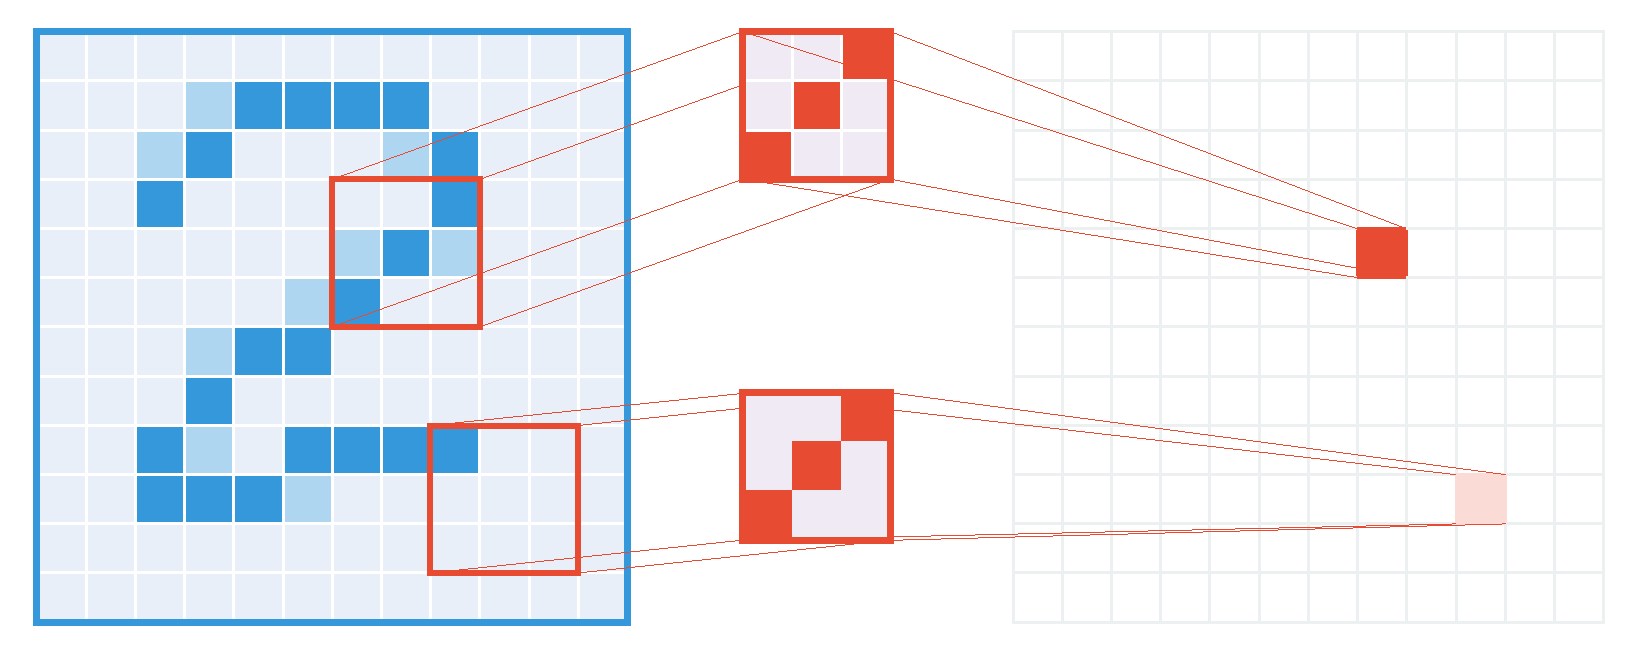
\includegraphics[width=0.8\textwidth]{images/convolution.pdf}
    \caption{ชั้นสังวัฒนาการ ซึ่งแสดงข้อมูลนำเข้าด้วยสีฟ้า และตัวกรองด้วยสีแดง}
    \label{conv-figure}
\end{figure}
\begin{figure}
    \centering
    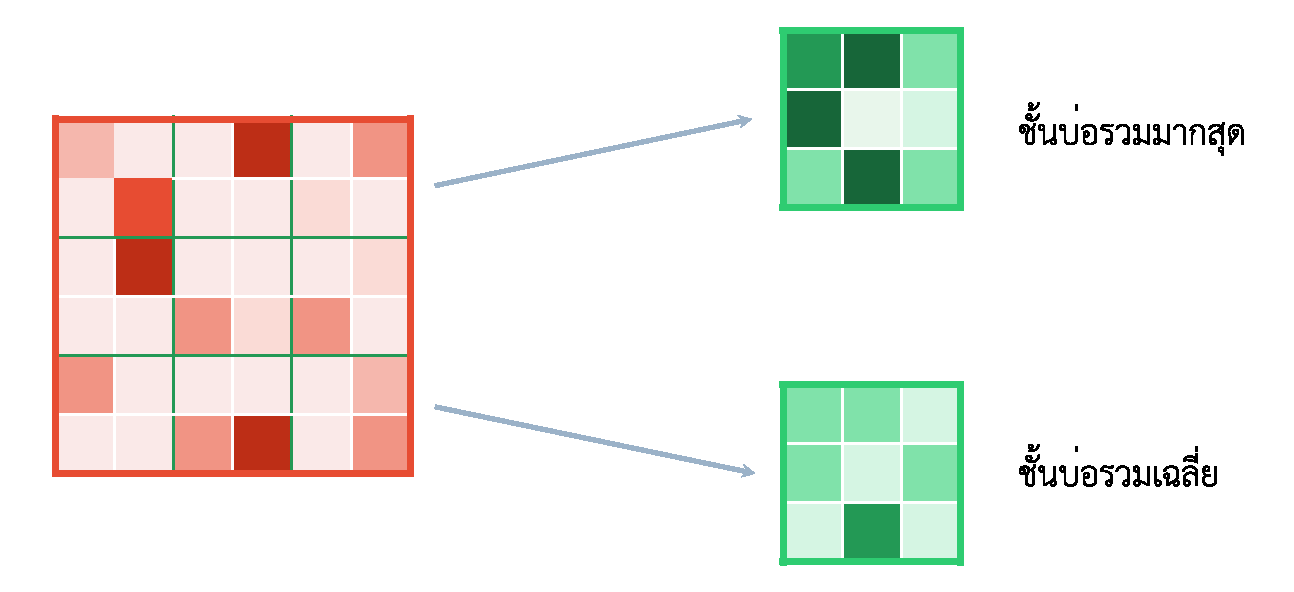
\includegraphics[width=0.8\textwidth]{images/pool.pdf}
    \caption{ชั้นบ่อรวม ทั้งแบบบ่อรวมมากสุดและแบบบ่อรวมเฉลี่ย โดยพิจารณาบ่อตามขอบเขตสีเขียว}
    \label{pool-figure}
\end{figure}
การสังวัฒนาการของชั้นสังวัฒนาการในโครงข่ายประสาทเทียม ทำหน้าที่เป็นตัวตรวจจับคุณสมบัติ (feature detector) เช่นการตรวจจับขอบ (edge detection) และชั้นบ่อรวมทำให้ขนาดของผลัพธ์จากชั้นสังวัฒนาการมีขนาดเล็กลง เพื่อให้จำนวนค่าน้ำหนักของโครงข่ายประสาทเทียมที่ต้องคำนวนนั้นน้อยลง

การเรียนรู้ด้วยวิธีก้าวเคลื่อนถอยหลัง (backpropagation learning) เป็นวิธีการเรียนรู้ที่ได้รับความนิยมมากที่สุดในปัจจุบัน ทั้งนี้ เราอาจพิจารณาการเรียนรู้ถอยหลังได้โดยทำความเข้าใจถึงฟังก์ชันสูญเสีย (loss function) และการปรับค่าตัวแปรเสริม (parameters) ดังนี้

\begin{figure}
    \centering
    \def\layersep{2.5cm}
    \begin{tikzpicture}[->,draw=black!70, node distance=\layersep]
        \tikzstyle{every pin edge}=[<-,shorten <=1pt]
        \tikzstyle{neuron}=[circle,draw=black!100,minimum size=17pt, outer sep=3pt]
        \tikzstyle{annot}=[text width=5em, text centered]
    
        \foreach \name / \y in {1,...,4}
            \node[neuron, pin=left:ข้อมูลรับเข้า \y] (I-\name) at (0,-\y) {};
    
        % Draw the hidden layer nodes
        \foreach \name / \y in {1,...,5}
            \path[yshift=0.5cm]
                node[neuron] (HA-\name) at (\layersep,-\y cm) {};
    
        \path[yshift=-1.5cm] node[neuron, fill=black!10] (O-1) at (2*\layersep,0 cm) {};
        \path[yshift=-1.5cm] node[neuron, fill=black!70] (O-2) at (2*\layersep,-1 cm) {};
        \path[yshift=-1.5cm] node[neuron, fill=black!20] (O-3) at (2*\layersep,-2 cm) {};
    
        \path[yshift=-1.5cm] node[neuron, fill=black!0] (T-1) at (3.5*\layersep,0 cm) {};
        \path[yshift=-1.5cm] node[neuron, fill=black!100] (T-2) at (3.5*\layersep,-1 cm) {};
        \path[yshift=-1.5cm] node[neuron, fill=black!00] (T-3) at (3.5*\layersep,-2 cm) {};

        \foreach \source in {1,...,4}
            \foreach \dest in {1,...,5}
                \path (I-\source) edge (HA-\dest);
    
        \foreach \source in {1,...,5}
            \foreach \dest in {1,...,3}
                \path (HA-\source) edge (O-\dest);

        \foreach \dest in {1,...,2}
            \path [<->] (T-\dest) edge (O-\dest);
        \draw [<->] (T-3) -- (O-3) node [midway, below] (losstext) {คำนวนค่าสูญเสีย};

        \node[annot,above of=I-1, node distance=1cm] (hla) {ชั้นรับเข้า};
        \node[annot,above of=HA-1, node distance=1cm] (hla) {ชั้นซ่อน};
        \node[annot,above of=O-1, node distance=1cm] (hlo) {ชั้นส่งออก};
        \node[annot,above of=T-1, node distance=1cm] (hlt) {คำตอบจริง};
    \end{tikzpicture}
    \caption{การคำนวนค่าสูญเสีย}
    \label{loss}
\end{figure}

\section{ค่าสูญเสีย}

ค่าสูญเสีย (loss) เป็นค่าที่ใช้ในการบอกว่าแบบจำลองใดๆ ตอบผิดมากหรือน้อยเพียงใด โดยค่าสูญเสียยิ่งมาก หมายถึงแบบจำลองตอบผิดมากเท่านั้น

ยกตัวอย่างเช่น หากเราสร้างแบบจำลองที่ต้องการส่งออกค่าเป็นค่าในลักษณะของการเข้ารหัสแบบหนึ่งจุดร้อน (one-hot encoding) ของค่าที่เป็นไปได้ 3 ชั้น (classes) จากข้อมูลตัวที่ i บนชุดฝึกหัด ดังแสดงในรูปที่ \ref{loss} ซึ่งต้องการคำตอบ $t_i$ ที่ถูกต้องเป็น
$$t_i = 
\begin{bmatrix}
    0 & 1 & 0
\end{bmatrix}
$$
ทว่า แบบจำลองกลับให้คำตอบ $o_i$ จากแบบจำลองเป็น
$$o_i = 
\begin{bmatrix}
    0.1 & 0.7 & 0.2
\end{bmatrix}
$$
เราอาจนิยามฟังก์ชันสูญเสียอย่างง่าย เพื่อยกตัวอย่างการคำนวนดังกล่าว โดยกำหนดให้ฟังก์ชันสูญเสียเป็นผลรวมของผลต่างกำลังสอง

$$
l_i\left(t_i, o_i\right) = \sum_{j=1}^{n}{\left(t_i[j] - o_i[j]\right)^2}
$$
ดังนั้น ในกรณีนี้ จะได้ค่าสูญเสียของจุดฝึกหัดนี้เป็น
\begin{align*}
    l_i\left(t_i, o_i\right) &= \sum_{j=1}^{n}{\left(t_i[j] - o_i[j]\right)^2}\\
    &= \left((0-0.1)^2 + (1-0.7)^2 + (0-0.2)^2\right)
\end{align*}
จะเห็นว่า ยิ่งค่า $t_i$ ใกล้เคียง $o_i$ มากขึ้นเท่าใด ค่าสูญเสียก็จะน้อยลงเท่านั้น

นอกจากนี้ เราจะนิยามค่าสูญเสียบนชุดฝึกหัดทั้งชุด เป็น
\begin{equation}
\mathscr{L}(T, O) = \sum_{i=1}^{N} l_i(t_i, o_i)
\end{equation}
เมื่อ $T$ และ $O$ เป็นชุดคำตอบ และค่าส่งออกจากแบบจำลองของทั้งชุดฝึกหัด ซึ่งชุดฝึกหัดมีความยาวเป็น $N$

อย่างไรก็ตาม ฟังก์ชันสูญเสียในลักษณะดังกล่าว เป็นฟังก์ชันอย่างง่าย ในการฝึกสอนแบบจำลองทั่วไปมักนิยมใช้ฟังก์ชันอื่น เช่นค่าสูญเสียแบบความวุ่นวายข้ามชั้น (cross entropy loss) สำหรับการฝึกสอนแบบจำลองเพื่อการทำการจำแนกหมวดหมู่ (classification)
$$
    \ell_i = -\sum_{c=1}^{M}y_{o,c}\ln(p_{o,c})
    \label{cross-entropy-loss}
$$
เมื่อ $M$ เป็นจำนวนชั้น (class) ที่เป็นไปได้ $y$ เป็นค่าฐานสองที่บ่งบอกว่าชั้นข้อมูล (class) $c$ เป็นคำตอบที่ถูกต้องสำหรับการคาดเดา (observation) $o$ และ $p$ เป็นค่าความน่าจะเป็นที่การคาดเดา $o$ ตอบว่าเป็นชั้นข้อมูล $c$

\subsection{ค่าสูญเสียเมื่อมองจากมุมมองของตัวแปรเสริม}
สมการที่นำเสนอไปข้างต้น มองค่าสูญเสียเปลี่ยนไป เมื่อใส่ชุดของข้อมูลส่งออกจากแบบจำลอง $O$ และค่าคำตอบจริง $T$ ต่างกันออกไป ทว่า หากพิจารณาว่า
\begin{itemize}
    \item แบบจำลองใดๆ สามารถปรับค่าตัวแปรเสริม (parameters) ได้อย่างอิสระ
    \item ค่าส่งออก $O$ เป็นฟังก์ชันของค่ารับเข้า $I$ โดย $O = f(I)$ เมื่อ $f$ เป็นฟังก์ชันของโครงข่ายประสาทเทียม
    \item ความมุ่งหมายฝึกสอนแบบจำลองใดๆ ให้มีประสิทธิภาพ อยู่บนการฝึกสอนบนชุดของค่าคำตอบจริง $T$ เดิม
\end{itemize}
เราจะสามารมองฟังก์ชันสูญเสีย เป็นฟังก์ชันที่รับค่าตัวแปรเสริม (กล่าวคือค่าน้ำหนักและอคติของแบบจำลอง) และส่งออกค่าสูญเสียของชุดตัวแปรเสริมนั้น

กล่าวอีกนัย หากเรามีชุดของตัวแปรเสริม $\vec{\theta}_1, \vec{\theta}_2, \dots, \vec{\theta}_i$ บนโครงสร้างของแบบจำลองการเรียนรู้เชิงลึก (deep learning models) ที่มีโครงสร้างเหมือนกัน เราอาจพิจารณาค่าฟังก์ชันสูญเสีย $\mathscr{L}(\vec{\theta}_i)$ บนชุดตัวแปรเสริม $\vec{\theta}_i$ และกล่าวว่าแบบจำลองที่ใช้ชุดตัวแปรเสริม $\vec{\theta}_i$ นั้นทำงานได้ดีกว่า $\vec{\theta}_j$ หาก $\mathscr{L}(\vec{\theta}_i) < \mathscr{L}(\vec{\theta}_j)$ 

\section{ขั้นตอนวิธีเกรเดียนต์ลดหลั่น และการก้าวเคลื่อนถอยหลัง}

\subsection{ตัวดำเนินการเกรเดียนต์}

พิจารณาตัวดำเนินการเกรเดียนต์ ซึ่งดำเนินการบนเวกเตอร์ใดๆ

\begin{definition}
    \textbf{เกรเดียนต์} ของฟังก์ชัน $f(\vec{x})$ ซึ่งเป็นฟังก์ชันของชุดตัวแปร $\vec{x} = \left(x_1, x_2, \dots, x_n\right)$ ใดๆ จะถูกนิยามเป็นตัวดำเนินการ $\vec{\nabla}f\left(\vec{x}\right)$
    $$
        \vec{\nabla}f\left(\vec{x}\right) = \sum_{i=1}^{n} \frac{\partial}{\partial x_i} \left( f(\vec{x}) \cdot \hat{x_i} \right) 
    $$
    เมื่อ $\hat{x_i}$ เป็นเวกเตอร์หนึ่งหน่วย (unit vector) ตามแกนของ $x_i$
\end{definition}
กรุณาสังเกตว่า ทิศทางของเกรเดียนต์นั้นจะชี้ไปในทิศทางที่เพิ่มขึ้นของฟังก์ชันเสมอ

เมื่อพิจารณาฟังก์ชันสูญเสีย ซึ่งเป็นฟังก์ชันที่เราต้องการลดค่า เราอาจพิจารณาหาค่าที่น้อยลงของฟังก์ชันได้ ด้วยการคำนวนเกรเดียนต์ของฟังก์ชันสูญเสียใดๆ แล้ว ``เดิน''  ไปในทิศทางตรงข้ามกับเกรเดียนต์ เปรียบประหนึ่งการเดินลงเขา ขั้นตอนวิธีดังกล่าวเรียกว่าขั้นตอนวิธีเกรเดียนต์ลดหลั่น (gradient descent algorithm) โดยพิจารณาการปรับแบบจำลองอยู่บนเกรเดียนต์ของฟังก์ชันสูญเสีย
\begin{equation}
    \vec{\theta}' = \vec{\theta} - l \vec{\nabla}{\mathscr{L}(\vec{\theta})}
    \label{gradient-descent}
\end{equation}
เมื่อ $l$ เป็นค่าอัตราการเรียนรู้ (learning rate) โดยปกติมักมีค่าไม่มาก

\begin{algorithm} 
    \caption{ขั้นตอนวิธีเกรเดียนต์ลดหลั่นเพื่อการฝึกสอนแบบจำลอง}
    \label{train-model}
    \begin{algorithmic}
        \STATE ประกาศตัวแปร $\hat{\theta}$ เป็นค่าสุ่มของเวกเตอร์ความยาวเท่าตัวแปรเสริมที่แบบจำลอง $M$ ต้องการ
        \FOR{$i=0$ ถึง $N$}
            \STATE คำนวนหาเกรเดียนต์ของ $\vec{\theta}$ โดย 
            $$
                \vec{\nabla}{\mathscr{L}(\vec{\theta})}
            $$
            \STATE ปรับค่า $\vec{\theta}$ โดย
            $$
                \vec{\theta}' = \vec{\theta} - l \vec{\nabla}{\mathscr{L}(\vec{\theta})}
            $$
        \ENDFOR
        \STATE ส่งคืนค่า $\vec{\theta}$
    \end{algorithmic}
\end{algorithm}

รหัสเทียมของขั้นตอนวิธีดังกล่าวสามารถศึกษาได้จากขั้นตอนวิธี \ref{train-model}

หากอธิบายโดยคร่าว ขั้นตอนวิธีเกรเดียนต์ลดหลั่น พยายามหาค่าตัวแปรเสริม $\theta_{\textrm{OPT}}$ โดยการเริ่มจากการสุ่มตัวแปรเสริม $\theta$ แล้วคำนวนเกรเดียนต์ของฟังก์ชันสูญเสีย และค่อยๆ ปรับค่า $\theta$ ตามทิศตรงข้ามกับเกรเดียนต์เรื่อยๆ จนกระทั่งถึงจุดที่ฟังก์ชันสูญเสียมีค่าน้อยที่สุด

\subsection{ขั้นตอนวิธีก้าวเคลื่อนถอยหลัง}

หนึ่งในประเด็นสำคัญที่จำเป็นต้องกล่าวถึงต่อมา คือวิธีการในการคำนวนเกรเดียนต์ $\vec{\nabla}(\vec{x})$ ซึ่งจำเป็นต้องคำนวนอนุพันธ์ (derivation) ของตัวแปรเสริมใดๆ เทียบกับฟังก์ชันสูญเสีย พึงพิจารณาว่าตัวแปรเสริมของแบบจำลองการเรียนรู้เชิงลึก คือชุดน้ำหนักและค่าอติต่างๆ

อย่างไรก็ตาม การคำนวนเกรเดียนต์และอนุพันธ์ดังกล่าวสามารถทำได้โดยง่าย ผ่านการใช้กฎลูกโซ่ (chain rule) ซึ่งนิยามได้ว่า
\begin{equation}
    \frac{dy}{dx} = \frac{dy}{du} \cdot \frac{du}{dx}
    \label{chain-rule}
\end{equation}
ในเล่มรายงานนี้จะไม่ลงรายละเอียดถึงขั้นตอนวิธีก้าวเคลื่อนถอยหลัง อย่างไรก็ดี สามารถพิจารณาได้ว่า (1) อนุพันธ์ของฟังก์ชันสูญเสียกับน้ำหนักของชั้นส่งออกสามารถพิจารณาได้โดยตรง และ (2) อนุพันธ์ของฟังก์ชันสูญเสียกับน้ำหนักของชั้นซ่อนใดๆ สามารถพิจารณาได้จากกฎลูกโซ่ดังสมการที่ \ref{chain-rule} เป็นผลคูณของอนุพันธ์ของฟังก์ชันสูญเสียเทียบกับน้ำหนักของชั้นส่งออก และอนุพันธ์ของน้ำหนักชั้นส่งออกเทียบกับชั้นซ่อน

\section{สัญญาณรบกวน}

การโจมตีแบจำลองการเรียนรู้เชิงลึกด้วยการหาสัญญาณรบกวน $\eta$ ที่โจมตีแบบจำลองการเรียนรู้ $M$ นั้นมีจุดประสงค์หลักคือหาค่า $\eta$ ซึ่งอยู่บนโดเมนเดียวกับข้อมูลรับเข้าโครงข่ายประสาทเทียม ที่ทำการเพิ่มค่าของฟังก์ชั่นสูญเสียจนถึงขีดสุด

เราจะเรียก $x' = x+\eta$ ว่าเป็น\textbf{ตัวอย่างประสงค์ร้าย (adversarial example)} เนื่องจากเป็นตัวอย่างที่ทำให้ค่าสูญเสียของโครงข่ายประสาทเทียมเพิ่มสูงขึ้นที่สุด

การหาสัญญาณรบกวนอาจมองเป็นปัญหาการเพิ่มประสิทธิภาพสูงสุด (optimisation problem) โดยพิจารณาการหา
\begin{equation}
    \eta = \epsilon \mathrm{argmax}\mathscr{L}\left(x+\eta, y\right)
    \label{perturbation}
\end{equation}
เมื่อคู่อันดับ $(x,y)$ แทนที่ตำแหน่งของชุดข้อมูลฝึกหัด (training point) หนึ่งจุด

ทั้งนี้ทั้งนั้น ขนาด (norm) ของ $\eta$ จะต้องมีค่าน้อยเพียงพอเมื่อเทียบกับ $x$ เพื่อทำให้\textit{ความเข้ม}ของสัญญาณรบกวนไม่เข้มจนเกินไปจนสามารถแยกแยะด้วยตาของมนุษย์ได้ว่าเป็นภาพที่ถูกเจือด้วยสัญญาณรบกวน ดังเช่นแสดงในรูปที่ \ref{perturbation-density}

\begin{figure}
    \centering
    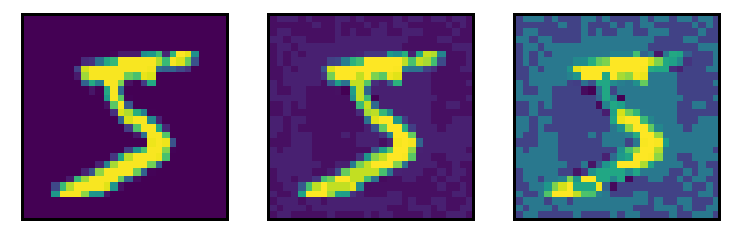
\includegraphics[width=0.7\textwidth]{images/density.pdf}
    \caption{(จากซ้ายไปขวา) รูปเลข 5 ที่ถูกเจือด้วยความเข้มข้นของสัญญาณรบกวนที่ต่างกันที่ระดับ 0.0,  0.01 และ 0.03 ตามลำดับ}
    \label{perturbation-density}
\end{figure}

\section{คำอธิบายต่อการเกิดขึ้นของสัญญาณรบกวน}

มีหลายทฤษฎีพยายามอธิบายการเกิดขึ้นของการโจมตีแบบจำลอง ซึ่งอาจยกตัวอย่างทฤษฎีและคำอธิบายได้ดังนี้

\subsection{การประพฤติตัวเป็นเส้นตรง}
LeCun และคณะ \cite{1412.6572} ศึกษาผลของการโจมตีที่เกิดจาก $\tilde{x}$ โดยอาจพิจารณาได้จากการคูณสมการเพื่อหาค่าส่งออกจากชุดน้ำหนัก (weights) ของชั้นแบบจำลองการเรียนรู้เชิงลึก (deep learning layers) 
\begin{equation}
    w^\top\tilde{x} = w^\top x + w^\top \eta
\end{equation}
คณะวิจัยสังเกตพฤติกรรมว่าสัญญาณรบกวน $\eta$ กระตุ้นส่วนของชุดน้ำหนักและฟังก์ชันกระตุ้น (activation function) ในแบบจำลองให้ประพฤติตัวเยี่ยงฟังก์ชันเส้นตรง (linear functions) ซึ่งการแสดงพฤติกรรมดั่งเส้นตรง (linearity) ในกรณีชายขอบ (edge case) ของข้อมูลรับเข้านั้นก่อให้เกิดความเป็นไปได้ที่แบบจำลองจะถูกโจมตี

เพื่อพิสูจน์ทฤษฎีดังกล่าว LeCun และคณะ พิจารณาผลความน่าจะเป็นของคำตอบที่ออกจากแบบจำลองเมื่อปรับค่า $\epsilon$ ดังแสดงในสมการที่ \ref{perturbation} และพบว่าความน่าจะเป็นของข้อมูลส่งออก (output) ของแต่ละชั้นข้อมูล (class) มีความสัมพันธ์เชิงเส้นตรงกับค่า $\epsilon$ ที่เพิ่มขึ้นเรื่อยๆ

\subsection{ทฤษฎีชุดคุณสมบัติแบบอ่อนและแบบเข้ม}

\begin{figure}
    \centering
    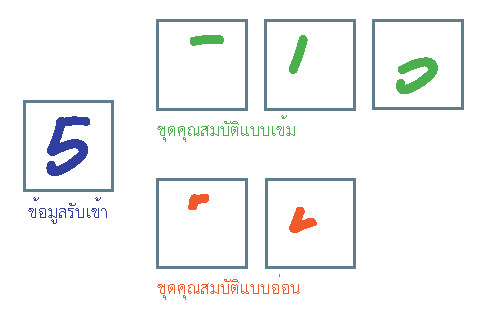
\includegraphics[width=0.5\textwidth]{images/strong-weak-features.pdf}
    \caption{ตัวอย่างชุดคุณสมบัติแบบอ่อน และแบบเข้มที่เป็นไปได้ จากเลข 5}
    \label{5-weak-strong}
\end{figure}

Ilyas และคณะ \cite{1905.02175} ศึกษาโครงสร้างของแบบจำลองเชิงลึก จนนำมาสู่ข้อสรุปว่า ``ช่องโหว่ในการโจมตีแบบจำลองเป็นผลโดยตรงจากความอ่อนไหวของแบบจำลองในการวางหลักการบนชุดคุณสมบัติของข้อมูล" (``Adversarial vulnerability is a direct result of our models’ sensitivity to well-generalizing features in the data")

หากกล่าวให้ละเอียด พิจารณาว่าโครงสร้างของแบบจำลองเชิงลึกสามารถเรียนรู้ชุดคุณสมบัติ (features) ของข้อมูลรับเข้าได้สองแบบ ซึ่งในงานวิจัยเรียกว่าชุดคุณสมบัติแบบอ่อน (weak features) และชุดคุณสมบัติแบบเข้ม (strong features)

\begin{itemize}
    \item ชุดคุณสมบัติแบบเข้ม คือชุดคุณสมบัติที่มนุษย์มองเห็นโดยทั่วไป กล่าวคือเป็นชุดคุณสมบัติที่มนุษย์สามารถสังเกต ทำความเข้าใจ และวางหลักการในการจำแนกได้
    \item ชุดคุณสมบัติแบบอ่อน คือชุดคุณสมบัติที่มนุษย์ไม่สามารถมองเห็น หรือมองเห็นแต่ไม่ได้หยิบมาเป็นตัวปัจจัยหลักในการตัดสินใจ และวางหลักการในการจำแนก
\end{itemize}

จะยกตัวอย่างกรณีการจำแนกเลข 5 เราอาจพิจารณาว่าเลข 5 ดังแสดงในรูปที่ \ref{5-weak-strong} ประกอบขึ้นจากขีดหนึ่งขีดแนวขวาง ขีดหนึ่งขีดแนวตั้ง และส่วนโค้งคล้ายวงกลม เป็นชุดคุุณสมบัติที่มนุษย์สังเกตและเข้าใจโดยทั่วไป รวมถึงเป็นคุณสมบัติที่มนุษย์ใช้ในการสังเกตเห็นเส้นที่เชื่อมต่อกันจนประกอบเป็นเลข 5 อย่างไรก็ตาม แบบจำลองการเรียนรู้ใดๆ อาจเห็นมุมรอยต่อระหว่างขอบ (ซึ่งอาจสังเกตได้ว่าไม่มีเลขตัวใดเลยนอกจาก 1 ถึง 9 ยกเว้น 5 ที่มีมุมและขอบดังแสดง) เป็นตัวตัดสินใจในการเรียนรู้เลข 5 อย่างไรก็ตาม พึงสังเกตว่าแบบจำลองอาจจะแม้กระทั่งเลือกสังเกตเห็นพื้นที่ว่างบริเวณที่แตกต่างกันไป และใช้พื้นที่ว่างเหล่านั้นเพื่อสร้างข้อสรุปหรือตัดสินใจว่าเลขที่มองเห็นเป็นเลขใด (ซึ่งการนำมาซึ่ง ``ข้อสรุป'' จากที่ว่างนั้น ขัดกับวิสัยปกติของมนุษย์ในการสังเกตและมองเห็นอย่างชัดเจน)

\section{การคำนวนหาสัญญาณรบกวน}

ขั้นตอนวิธีการหาสัญญาณรบกวนนั้นมีรายละเอียดต่างกันออกไปตามวิธีการคำนวน และแนวคิดของการคำนวน ดังแสดงตัวอย่างวิธีต่อไปนี้

\subsection{การหาสัญญาณรบกวนด้วยวิธีการก้าวเคลื่อนถอยหลัง}
เมื่อฝึกสอนแบบจำลองการเรียนรู้เชิงลึกโดยได้ชุดตัวแปรเสริม $\theta$ สำหรับแบบจำลอง $M$ ซึ่งต่อไปนี้จะเรียกชุดแบบจำลองและตัวแปรเสริมรวมกันว่า $M_\theta$ แล้ว เมื่อให้คู่จุดข้อมูลรับเข้าและส่งออก $(x, y)$ ใดๆ เราอาจหาสัญญาณรบกวนได้ว่า
\begin{equation}
    \eta' = \eta + l \frac{\partial}{\partial \eta} \mathscr{L}\left( x \right)
    \label{adver-gradient-descent}
\end{equation}
เมื่อ $l$ เป็นค่าอัตราการเรียนรู้ (learning rate) โดยปกติมักมีค่าไม่มาก

จะสังเกตได้ว่าสมการที่ \ref{adver-gradient-descent} มีลักษณะคล้ายกับสมการที่ \ref{gradient-descent} เป็นอย่างมาก แตกต่างกันเพียงแต่เครื่องหมายบวกหรือลบ และตัวแปรเทียบสำหรับการทำอนุพันธ์หลายตัวแปร (multivariable derivation) ขอให้สังเกตว่าในขณะที่สมการ \ref{gradient-descent} พยายามหาค่า $\theta$ ที่ทำให้ฟังก์ชันสูญเสีย $\mathscr{L}$ มีค่าต่ำที่สุด สมการที่ \ref{adver-gradient-descent} กลับพยายามหาสัญญาณรบกวน $\eta$ ที่ทำให้ฟังก์ชันสูญเสีย $\mathscr{L}$ มีค่ามากที่สุด กล่าวคือตอบผิดมากที่สุด

\subsection{การหาสัญญาณรบกวนด้วยวิธีการเครื่องหมายเกรเดียนต์แบบเร็ว (FGSM)}

Goodfellow และคณะ \cite{1412.6572} ได้เสนอขั้นตอนวิธีสำหรับคำนวนหาสัญญาณรบกวน $\eta$ สำหรับชุดคู่จุด $(x, y)$ โดยสังเกตทิศทางของเกรเดียนต์ของฟังก์ชันสูญเสีย $\mathscr{L}$ เทียบกับ $x$ ซึ่งสามารถคำนวนได้จาก
\begin{equation}
    \eta = \epsilon \mathrm{sign} \left(\vec{\nabla}_x \mathscr{L}\left(\theta, x, y \right) \right)
\end{equation}
เรียกขั้นตอนวิธีนี้ว่า\textbf{วิธีการเครื่องหมายเกรเดียนต์แบบเร็ว (Fast Gradient Sign Method: FGSM)}

แนวคิดเบื้องหลังขั้นตอนวิธีนี้คือ เมื่อมีเกรเดียนต์ของฟังก์ชันสูญเสียต่อแบบจำลอง ทิศทางของเกรเดียนต์นั้นย่อมทำให้เกิดการเปลี่ยนแปลงต่อค่าของฟังก์ชันสูญเสียมากขึ้นที่สุด 

ค่าจากฟังก์ชัน sign นั้นจะเป็นค่าบวกหรือลบหนึ่ง กล่าวคือเราสนใจพิจารณาเฉพาะทิศทางของเกรเดียนต์ และจะทำการคูณค่านั้นด้วยค่าคงที่ $\epsilon$ เพื่อเจือสัญญาณรบกวนไม่ให้มีความเข้มข้นมากเกินไป

สังเกตว่าความซับซ้อนเชิงเวลา (time complexity) ของขั้นตอนวิธีนี้เป็น $\mathcal{O}(1)$ เพราะไม่มีการวนรอบซ้ำ

\subsection{การฉายเกรเดียนต์ลดหลั่น $k$ ขั้น ($k$-PGD)}

ขั้นตอนวิธี FGSM นั้นมีข้อดีในด้านเวลาการทำงาน อย่างไรก็ตาม การประมาณค่าของเกรเดียนต์ที่มากที่สุดโดยมิได้พิจารณาถึงพื้นผิวของฟังก์ชัน ยอมทำให้ค่าของเกรเดียนต์ที่ออกมานั้นผิดเพี้ยน และไม่ได้ค่าฟังก์ชันสูญเสียที่มากที่สุด ทำให้ไม่ใช่ชุดสัญญาณรบกวนที่ดีที่สุดที่จะโจมตีแบบจำลองได้

Madry และคณะ \cite{aleks2017deep} จึงศึกษาขั้นตอนวิธีที่ใช้การวนซ้ำเพื่อหาค่าของ $x' = x + \eta$ โดยมุ่งให้การวนซ้ำนั้นช่วยในการปรับค่าของ $\eta$ เพื่อเพิ่มค่าฟังก์ชันสูญเสียอย่างแม่นยำ โดยปรับค่าของ $x'$ ในแต่ละรอบ $t$ ได้จากสมการ
\begin{equation}
    x'_t = \text{Proj}_{x'}^\epsilon(x_{t-1} +\alpha \vec{\nabla}_{x_{t-1}}\mathscr{L}(x_{t-1}))
\end{equation}
เมื่อ $x_0 = x$

ขั้นตอนวิธีดังกล่าวเรียกว่าขั้นตอนวิธี\textbf{การฉายเกรเดียนต์ลดหลั่น $k$ ขั้น ($k$-Projected Gradient Descent: $k$-PGD)} โดยจะวนซ้ำขั้นตอนนี้เป็นจำนวน $k$ ครั้ง จะสักเกตว่าทุกรอบการวนซ้ำจะทำการฉาย (project) ทิศทางของเกรเดียนต์ของฟังก์ชันสูญเสียออกไปเป็นระยะทาง $\alpha$ และฉายกลับเข้ามายังกรอบ $\epsilon$ ที่กำหนดไว้หากขนาดของสัญญาณรบกวนมีค่าเกินตามต้องการ

\subsection{ความต่างของขั้นตอนวิธี}

แม้ว่าขั้นตอนวิธี $k$-PGD จะทำงานได้ช้า แต่การทำงานที่เป็นแบบการวนซ้ำ (iteratively) ช่วยให้มั่นใจว่าการเพิ่มขึ้นของสัญญาณรบกวนจากเกรเดียนต์เป็นไปได้อย่างแม่นยำและสร้างความเสียหายใจการโจมตีได้มาก

ในขณะเดียวกัน ขั้นตอนวิธี FGSM แม้จะไม่สามารถสร้างสัญยาณโจมตีที่มีประสิทธิภาพ แต่ก็สามารถสร้างสัญญาณโจมตีที่โจมตีในกรณีทั่วไปได้ และสร้างได้อย่างรวดเร็ว

\section{การเรียนรู้เชิงโจมตี}

การเรียนรู้เชิงโจมตีเป็นขั้นตอนวิธีหนึ่งในการเสริมความทนทานต่อการโจมตีให้แบบจำลองการเรียนรู้เชิงลึก ขั้นตอนวิธีการเรียนรู้เชิงโจมตีที่ง่ายที่สุดคือการสร้างชุดข้อมูลประสงค์ร้ายและนำไปฝึกสอนร่วมกับชุดข้อมูลฝึกหัดตั้งต้น ดังแสดงใน

\begin{algorithm} 
    \caption{การเสริมความแข็งแกร่ง (การเรียนรู้เชิงโจมตี)}
    \label{retrain}
    \begin{algorithmic}
        \REQUIRE $M$ เป็นแบบจำลองการเรียนรู้
        \REQUIRE $X$ เป็นชุดข้อมูลที่จะทำการโจมตี
        \REQUIRE $e$ เป็นจำนวนรอบการวนซ้ำ (epoches) ในการฝึกสอน
        \REQUIRE $m$ และ $n$ เป็นขนาดของชุดฝึกสอนเล็กจิ๋ว (minibatch) บนชุดข้อมูลต้นฉบับและชุดข้อมูลประสงค์ร้าย
        \FOR{$i=1$ ถึง $e$}
            \STATE สร้างชุดฝึกสอนจิ๋วบนชุดข้อมูลต้นฉบับ $B=\{x_1, x_2, \dots, x_m\}$.
            \STATE สร้างชุดฝึกสอนจิ๋วบนชุดข้อมูลประสงค์ร้าย $B'=\{x_1', x_2', \dots, x_n'\}$.
            \STATE ฝึกสอนแบบจำลองด้วยชุดฝึกสอนเล็กจิ๋ว $B$ และ $B'$
        \ENDFOR
        \RETURN แบบจำลอง $M$
    \end{algorithmic}
\end{algorithm}

% \begin{algorithm}
%     \begin{algorithmic}
%          \STATE <text>
%     \end{algorithmic}
% \end{algorithm}

\chapter{วิธีดำเนินงาน}

\section{การวิเคราะห์และออกแบบขั้นตอนวิธี}

โครงงานวิศวกรรมคอมพิวเตอร์ชิ้นนี้มุ่งเสนอแนวคิดสำหรับการวิเคราะห์คลัสเตอร์เพื่อโจมตีแบบจำลองและใช้การโจมตีนั้นในการสอนแบบจำลองให้ทนทานต่อการโจมตี โดยตั้งอยู่บนแนวติดและสมมติฐานต่อไปนี้

\subsection{พฤติกรรมของคลัสเตอร์สัญญาณรบกวน}

หนึ่งในปัญหาของขั้นตอนวิธีเสริมความแข็งแกร่งแบบจำลอง คือการสร้างชุดสัญญาณรบกวนเพื่อฝึกสอนนั้นกินเวลานาน แม้จะมีขั้นตอนวิธีที่คำนวนได้อย่างรวดเร็วเช่นขั้นตอนวิธี FGSM แต่ขั้นตอนวิธีที่ใช้เวลาคิดคำนวนเร็วไม่สามารถสร้างสัญญาณรบกวนที่มีประสิทธิภาพในการโจมตีแบบจำลอง และสัญญาณรบกวนดังกล่าวไม่สามารถใช้ฝึกสอนแบบจำลองให้ทนทานต่อการโจมตีได้ \cite{aleks2017deep}

เพื่อลดปัญหาดังกล่าว โครงงานชิ้นนี้มุ่งเสนอแนวคิดว่า

\begin{claim}
    \label{in-cluster-attack}
    เมื่อให้ชุดข้อมูลประสงค์ร้าย $X'$ ที่โจมตีชุดข้อมูล $X$ พฤติกรรมของสัญญาณรบกวน $\eta$ สามารถจัดเป็นกลุ่มย่อยๆ ได้ และการโจมตีในสมาชิกของกลุ่มย่อยสามารถเกิดขึ้นได้ด้วยชุดสัญญาณโจมตีอื่นๆ ในจุดกลุ่มนั้น
\end{claim}

\begin{claim}
    \label{slow-fast-same}
    ผลการจัดกลุ่มคลัสเตอร์สัญญาณรบกวน ไม่ว่าจะบนสัญญาณรบกวนที่ได้มาจากวิธีการใด จะมีสมาชิกของแต่ละคลัสเตอร์ใกล้เคียงกัน
\end{claim}

ด้วยข้อสมมติฐานที่ \ref{slow-fast-same} เราสามารถสร้างสัญญาณรบกวนด้วยขั้นตอนวิธีที่เร็วเพื่อสร้างคลัสเตอร์ของสัญญาณรบกวนได้ เมื่อประกอบกับข้อสมมติฐานที่ \ref{in-cluster-attack} เราสามารถใช้ความรู้ของคลัสเตอร์มาช่วยร่นเวลาในการโจมตีแบบจำลองได้

ขั้นตอนวิธี \ref{cluster-gen} เสนอการคลัสเตอร์ข้อมูล และพยายามสร้างสัญญาณโจมตีด้วยขั้นตอนวิธีที่แม่นยำเพียงหนึ่งสัญญาณต่อคลัสเตอร์  กล่าวคือขั้นตอนวิธีดังกล่าวเรียกใช้ฟังก์ชันสำหรับสร้างสัญญาณรบกวนที่รวดเร็วเพียงเพื่อจัดกลุ่มของสัญญาณรบกวน ก่อนจะทำการโจมตีอย่างแม่นยำด้วยขั้นตอนวิธีที่แม่นยำ (แต่ไม่มีประสิทธิภาพทางด้านเวลา) ต่อไป

\begin{algorithm} 
    \caption{ขั้นตอนวิธีสร้างสัญญาณรบกวนจากคลัสเตอร์}
    \label{cluster-gen}
    \begin{algorithmic}
        \REQUIRE $M$ เป็นแบบจำลองการเรียนรู้
        \REQUIRE $X$ เป็นชุดข้อมูลที่จะทำการโจมตี
        \REQUIRE $k$ เป็นจำนวนคลัสเตอร์
        \REQUIRE $f_s$ เป็นฟังก์ชันสร้างสัญญาณรบกวนที่รวดเร็ว
        \REQUIRE $f_e$ เป็นฟังก์ชันสร้างสัญญาณรบกวนที่มีประสิทธิภาพ
        \STATE สร้างชุดสัญญาณรบกวน $P_s$ ที่โจมตีแบบจำลอง $M$ บนชุดข้อมูล $X$ ด้วยขั้นตอนวิธี $f_s$
        \STATE วิเคราะห์คลัสเตอร์ด้วยขั้นตอนวิธี $k$-มีนส์ บน $P_s$ ด้วยจำนวนคลัสเตอร์ $k$ คลัสเตอร์
        \FOR{ทุกคลัสเตอร์ $c_i \in C$}
            \STATE สร้างสัญญาณรบกวน $p_i$ ที่มีความสามารถโจมตีทุกจุด $c_i$ บนแบบจำลอง $M$ ด้วยขั้นตอนวิธี $f_e$
            \STATE เก็บสัญญาณรบกวน $p_i$ และเซต $C_i$ ซึ่งมีสมาชิก $c_i$ ทุกตัวในคลัสเตอร์ $C$
        \ENDFOR
        \RETURN ค่า $p_i$ และ $c_i$ สำหรับทุก $i = 1$ ถึง $k$
    \end{algorithmic}
\end{algorithm}

\subsection{การเสริมความแข็งแกร่งด้วยวิธีการผสานคลัสเตอร์}

จากขั้นตอนวิธี \ref{cluster-gen} เราสามารถนำชุดสัญญาณโจมตีมาฝึกสอนแบบจำลองเพื่อเสริมความแข็งแกร่งได้ ดังแสดงในขั้นตอนวิธี \ref{cluster-retrain}

\begin{algorithm} 
    \caption{การเสริมความแข็งแกร่งด้วยวิธีการผสานคลัสเตอร์}
    \label{cluster-retrain}
    \begin{algorithmic}
        \REQUIRE $M$ เป็นแบบจำลองการเรียนรู้
        \REQUIRE $X$ เป็นชุดข้อมูลที่จะทำการโจมตี
        \REQUIRE $e$ เป็นจำนวนรอบการวนซ้ำ (epoches) ในการฝึกสอน
        \REQUIRE $m$ และ $n$ เป็นขนาดของชุดฝึกสอนเล็กจิ๋ว (minibatch) บนชุดข้อมูลต้นฉบับและชุดข้อมูลประสงค์ร้าย
        \REQUIRE $w$ และ $w'$ เป็นน้ำหนักของชุดฝึกสอนเล็กจิ๋ว (minibatch) บนชุดข้อมูลต้นฉบับและชุดข้อมูลประสงค์ร้าย
        \STATE สร้างสัญญาณรบกวนจากคลัสเตอร์ ที่โจมตีข้อมูล $X$ บนแบบจำลอง $M$ โดยใช้ขั้นตอนวิธี \ref{cluster-gen}.
        \FOR{$i=1$ ถึง $e$}
            \STATE สร้างชุดฝึกสอนจิ๋วบนชุดข้อมูลต้นฉบับ $B=\{x_1, x_2, \dots, x_m\}$.
            \STATE สร้างชุดฝึกสอนจิ๋วบนชุดข้อมูลประสงค์ร้าย $B'=\{x_1', x_2', \dots, x_n'\}$.
            \STATE ฝึกสอนแบบจำลองแบบถ่วงน้ำหนัก โดยให้น้ำหนัก $w$ บน $B$ และ $w'$ บน $B'$.
        \ENDFOR
        \RETURN แบบจำลอง $M$
    \end{algorithmic}
\end{algorithm}

\section{การทดลองวัดประสิทธิภาพ}

นอกจากการเสนอขั้นตอนวิธีแล้ว ผู้จัดทำมุ่งความสนใจไปยังวิธีการวัดประสิทธิภาพของขั้นตอนวิธีด้วยเช่นกัน

ผู้จัดทำโครงงานจัดทำชุดคำสั่งสำหรับขั้นตอนวิธีที่เสนอในโครงงานวิศวกรรมชิ้นนี้ บนไลบรารี (library) การเรียนรู้เชิงลึก PyTorch \cite{PyTorch2019}

ชุดคำสั่งทั้งหมดสามารถเข้าถึงออนไลน์ได้ผ่านระะควบคุมเวอร์ชัน (Software Version Control) GitHub ผ่านทาง \url{https://github.com/srakrnxKU/adversarial-project/}

\bibliography{references} 
\bibliographystyle{ieeetr}
\end{document}